\section{Проектирование и разработка программного средства} 
\label{sec:development}

\subsection{Проектирование архитектуры программного средства} 
\label{sec:development:arch}

С учетом того, что выбранным языком для разработки является С++, то приложение будет разрабатываться в объектно-ориентированном стиле. Суть такого стиля заключается в представлении программы в виде совокупности самодостаточных объектов. Каждый из объектов выполняет свою роль и имеет свойства и методы, посредством которых он может взаимодействовать с другими объектами. При этом программисту часто не обязательно знать, как устроен объект. Достаточно только знать сигнатуры методов и типы полей, таким образом упрощается разработка приложений большого размера и повышается эффективность тестирования: уже отлаженные объекты больше не нужно отлаживать.

Также в данном курсовом проекте будет использоваться подход модульного программирования, 
а именно организация программы как совокупности независимых блоков, называемых модулями, 
структура и поведение которых подчиняются определённым правилам. 
Использование модульного программирования позволяет упростить тестирование программы и обнаружение ошибок. 
Совокупность классов, выполняющая одну и ту же категорию задач, находится в отдельном модуле.

Следует отметить, что так как мониторинг должен выполняться максимально быстро и на низком уровне, то основные классы будут представлять из себя высокоуровневые обертки над Win32 API, которые будет необходимо реализовать.

Итоговое программное средство будет состоять из двух приложений: клиент, представляющий из себя приложение мониторинга пользовательского ввода и сервер, выполняющий роль приемника и сохранения информации, полученной от клиентов.

Задача сервера состоит в том, чтобы принимать все входящие запросы на соединение, получать данные, посылаемые клиентами и записывать их на диск. Для выполнения поставленной задачи сервер должен реализовывать следующий функционал:
\begin{itemize}
	\item Класс FileService -- файловую службу, которая будет предоставлять методы для логирования данных в файл. Для работы с файлами будет использоваться файловый поток вывода, так как он имеет встроенную буферизацию, что позволяет уменьшить нагрузку на диск.
	\item Цикл обработки сообщений, который будет использоваться для управления поведением сервера.
	\item Менеджер соединений, работающий в отдельном потоке. Это необходимо для того, чтобы сервер мог получать управляющие команды от владельца сервера. Менедженр соединений должен принимать все входящие соединения и запускать для каждого отдельный поток с обработчиком.
	\item Обработчик активного соединения, который будет использовать собственный экземпляр класса FileService. Задача обработчика будет заключатся в получении данных из установленного соединения и записи результатов на диск.
	\item Поддержка аргументов командной строки для первоначальной настройки.

\end{itemize} 

Задачей клиента является сбор информации о нажатых клавишах в требуемых окнах и последующая отправка логов на сервер. Для выполнения поставленной задачи клиент должен реализовывать следующий функционал:
\begin{itemize}
	\item Класс Filters, реализующий методы для фильтрации текста по заданных критериям. Его задачей будет определять стоит ли писать лог пользовательского ввода для конкретного окна. Таким образом можно будет отделить действительно важные данные: логин, пароль, номер банковской карты от информации, не представляющей никакой ценности: поисковые запросы, набор документа и прочее.
	\item Класс TcpClient, реализующий методы для работы с удаленным сервером. Его задачей будет является установка соединения, отправка данных и оповещение об отсутствии соединения. Данный класс должен являться высокоуровневой оберткой над функциями Win API для работы с сокетами (winsock2.h).
	\item Класс Concealment, реализующий методы для распространения и сокрытия вредоносной программы от пользователя. К таким методам можно отнести: копирование исполняемого файла в директорию на диске C:/, скрытие этой директории, запрет на удаление файла путём изменения политик доступа Windows а также добавление программы в автозагрузку путём добавления ключа в реестр.
	\item Класс Keylogger, реализующий основную логику отслеживания пользовательского ввода с учётом фильтров, предоставляемых классом Filters. Задачей этого класса будет перехват нажатых клавиш и активных окон, и преобразование полученных данных в удобный текстовый формат с последующей отправкой на сервер. При этом необходимо предусмотреть случай, когда подключиться к серверу не удаётся.
	\item Функция, определяющая наличие существующего экземпляра программного средства в памяти. Это необходимо для того, чтобы одновременно не работало 2 одинаковых программы, в чем нет никакого смысла.
	\item Обработчик сообщения WM\_CLOSE для корректного завершения работы программного средства в случае завершения работы зараженного компьютера. Задача обработчика состоит в том, чтобы отправить всю оставшуюся информацию из буфера на сервер. 
\end{itemize} 

Среди подходов для отслеживания клавиш можно выделить следующие:
\begin{itemize}
	\item Использование функции GetKeyboardState \cite{msdn_WinApiGetKeyboardState}.
	\item Использование функции GetKeyState в цикле \cite{msdn_WinApiGetKeyState}.
	\item Использование функции GetAsyncKeyState в цикле \cite{msdn_WinApiGetAsyncKeyState}.
	\item Использование глобального перехватчика (Hook) сообщений клавиатуры.
\end{itemize} 
Рассмотрим каждый из подходов и выберем наилучший.

GetKeyboardState возвращает состояние клавиатуры на момент вызова. Главным недостатком данного подхода является то, что невозможно определить порядок нажатых клавиш. Если пользователь нажмет 3 клавиши одновременно, то они будут записаны в том порядке, в котором будут идти их виртуальные коды. Данный подход негодится для проектируемого программного средства, так как не достигается требуемая точность отслеживания.

GetKeyState возвращает состояние одной клавиши для активного потока. Это означает, что с помощью данной функции невозможно определить, какие клавиши нажимаются в приложениях отличных от проектируемого, что противоречит самой сути проектируемого программного средства.

GetAsyncKeyState возвращает состояние одной клавиши независимо от потока. Эту функцию можно использовать для удовлетворения функциональных требований, сформированных на этапе анализа, однако она не является идеальным вариантом по нескольким причинам: данная функция не может корректно распознавать удерживаемые клавиши, что сразу отражается на точности отслеживания, также порядок записи логов отслеживаемых клавиш может не совпадать с реальным. Причиной не совпадения является тот факт, что данная функций будет выполнятся в цикле (периодический опрос). Если в данном цикле отсутствует Sleep, то приложение будет очень требовательно к ресурсам за счет постоянной прогонки в бесконечном цикле. Если добавить небольшое ожидание, то есть шанс того, что в момент этого самого ожидания пользователь нажмет клавишу, которую программное средство не сможет отследить. Также лог нажатых клавиш может содержать клавиши в неправильном порядке. Пример такого случая следующий: пользователь почти одновременно нажимает клавиши 'z' и 'a' на клавиатуре (сначала 'z', потом 'a'), программное средство в цикле начинает вызывать GetAsyncKeyState для каждой отслеживаемой клавиши, но так как код клавиши 'a' меньше чем клавиши 'z', то итоговый лог будет 'az', хотя клавиши были нажаты в обратном порядке. По этому ряду причин использовать GetAsyncKeyState для решения поставленной задачи не рекомендуется.

Использование глобального перехватчика сообщений является идеальным подходом для решения поставленной задачи. Отсутствует необходимость в ожидании, не происходит пустых вызовов, появляется возможность более гибкой обработки нажатых клавиш.

В рамках данного курсового проекта для отслеживания нажатых клавиш будет использоваться глобальный перехватчик сообщений клавиатуры.

\subsection{Схемы основных алгоритмов по ГОСТ 19.701-90} 
\label{sec:development:algos}

Алгоритм, устанавливающий запрет на удаление заданной папки представлен на рисунке \ref*{sec:development:algos:deletepolicy}. Учитывая специфику работы с политиками Windows через Win32 API, для изменения существующей политики необходимо получить ссылку на уже существующую политику, а затем объеденить ее со специально созданным ограничением. В результате получится новая политика, которую можно будет установить для произвольной папки.

\begin{figure}[!hb]
	\centering
	  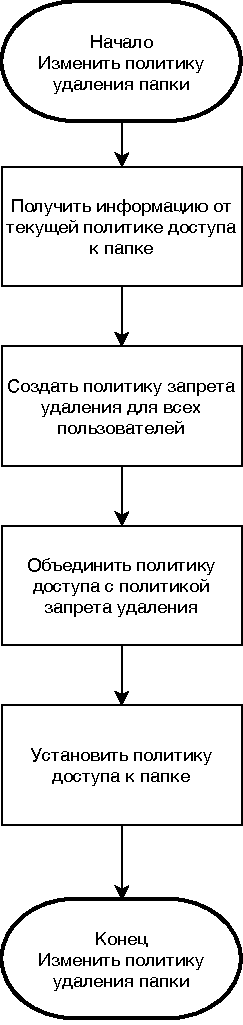
\includegraphics[scale=1]{attachments/DeletePolicy.pdf}  
	  \caption{ Алгоритм изменения политики удаления для папки }
	  \label{sec:development:algos:deletepolicy}
\end{figure}

Алгоритм подключение клиента к серверу с помощью функций Win32 API, представленных заголовочным файлом winsock2.h представлен на рисунке \ref*{sec:development:algos:clientconnect}. Алгоритм учитывает удачное и неудачное подключение, для того, чтобы вызывающий код мог определить результат выполнения метода. В качестве возвращаемого значения используется переменная типа BOOLEAN. 

\begin{figure}[hb]
	\centering
	  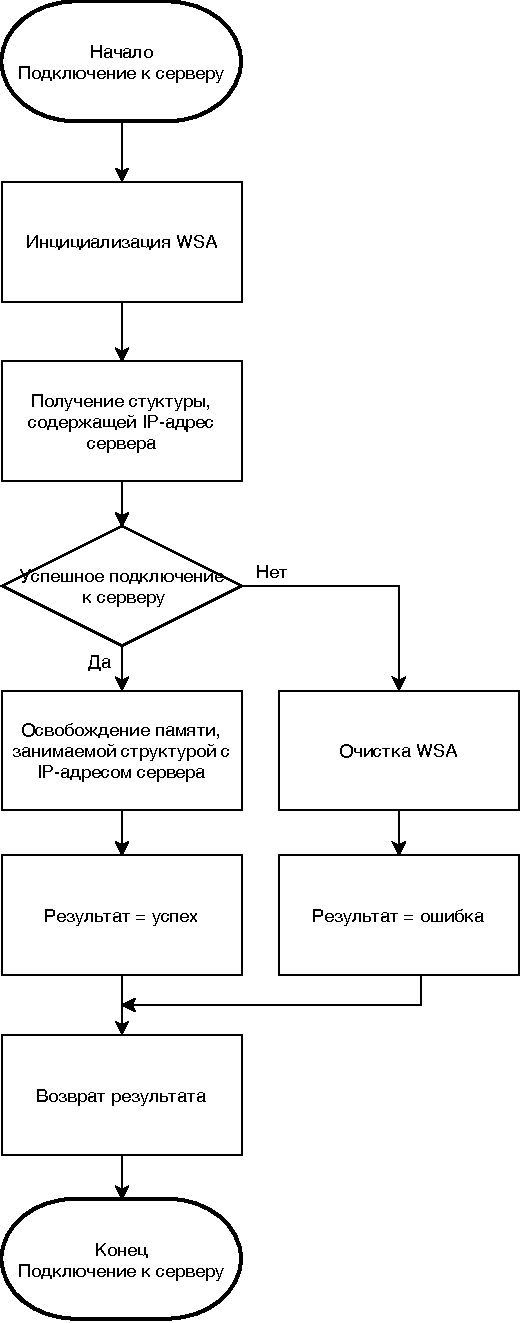
\includegraphics[scale=1]{attachments/ClientConnect.pdf}  
	  \caption{ Алгоритм подключения клиента к серверу }
	  \label{sec:development:algos:clientconnect}
\end{figure}

Алгоритм, проверяющий заданный массив клавиш на то, что они были нажаты в момент вызова представлен на рисунке \ref*{sec:development:algos:logkeys}. При этом для анализа значимости используется фильтрация по окнам. Таким образом получается избежать отправления не имеющей практического смысла информации на сервер. Для фильтрации используется класс Filter, а для отправки на сервер класс TcpClient.

\begin{figure}[hb]
	\centering
	  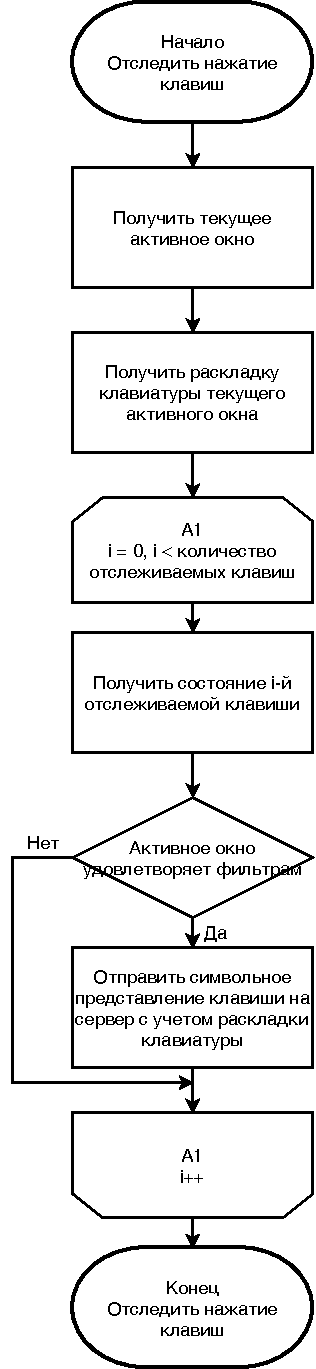
\includegraphics[scale=1]{attachments/LogKeys.pdf}  
	  \caption{ Алгоритм отслеживания нажатых клавиш }
	  \label{sec:development:algos:logkeys}
\end{figure}



Алгоритм начальной инициализации сервера с целью получения сокета для прослушки входящих соединений представлен на рисунке \ref*{sec:development:algos:initserver}. В дальнейшем данный сокет будет использоваться менеджером соединений для распределения обработчиков клиентов по разным потокам.

\begin{figure}[hb]
	\centering
	  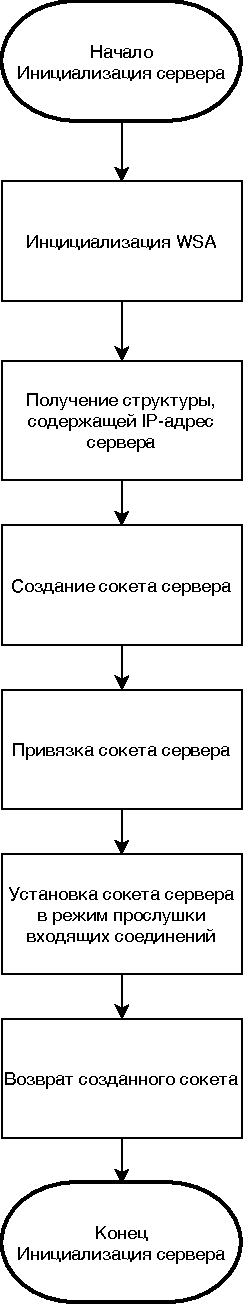
\includegraphics[scale=1]{attachments/InitServer.pdf}  
	  \caption{ Алгоритм инициализации сервера }
	  \label{sec:development:algos:initserver}
\end{figure}

Алгоритм принятия всех входящих соединении и распределения каждого в отдельный поток представлен на рисунке \ref*{sec:development:algos:connnectionmanager}. При этом дескрипторы потоков сохраняются. В случае, если сокет сервера больше не является активным, так как был произведен вызов CloseSocket или WSACleanup, то менеджер ожидает завершения всех порожденных потоков и освобождает ресурсы путем закрытия дескрипторов потоков.

\begin{figure}[!hbt]
	\centering
	  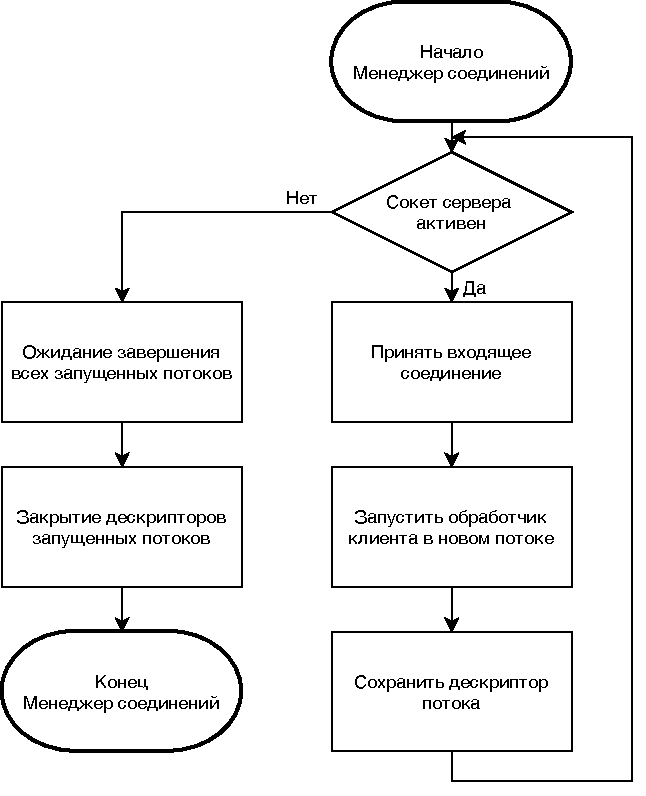
\includegraphics[scale=1.5]{attachments/ConnectionManager.pdf}  
	  \caption{ Алгоритм менеджера входящих соединений }
	  \label{sec:development:algos:connnectionmanager}
\end{figure}






